\chapter{Theoretical Background}
\label{chap:theoretical-background}

This chapter establishes the theoretical foundation necessary for understanding the design and implementation of the \ac{VMAP} database system. It begins with an overview of automotive electronic control systems and parameter management, explaining the fundamental concepts that drive the requirements for the \ac{VMAP} system. The chapter then explores database management systems, database design methodologies, and access control models relevant to the implementation. Finally, it discusses version control concepts and temporal database management approaches, which are critical for the parameter versioning requirements in automotive software development.

\section{Automotive Electronic Control Systems}
\label{sec:automotive-electronic-systems}

Modern commercial vehicles contain dozens of \acp{ECU} that manage various vehicle subsystems. Each \ac{ECU} is a specialized computing device that controls specific functions through software parameters \cite{staron2021automotive}. Understanding the structure and organization of these systems is essential for designing an effective parameter management solution.

\subsection{\ac{ECU} Hierarchy and Parameter Organization}
\label{subsec:ecu-hierarchy}

Automotive electronic systems follow a hierarchical organization that structures parameters into logical groupings. Figure \ref{fig:ecu-hierarchy} illustrates this hierarchical structure, showing how parameters are organized in automotive electronic systems. At the top level, \acp{ECU} represent distinct hardware components controlling specific vehicle functions such as engine management, transmission control, or brake systems \cite{kiencke2000automotive}. Within each \ac{ECU}, modules represent functional software units that implement specific capabilities such as cruise control, adaptive power steering, diagnosis. Each module contains \acp{PID} that group related parameters, and finally, individual parameters define specific configuration values that affect system behavior \cite{staron2021autosar}.

\begin{figure}[ht]
    \centering
    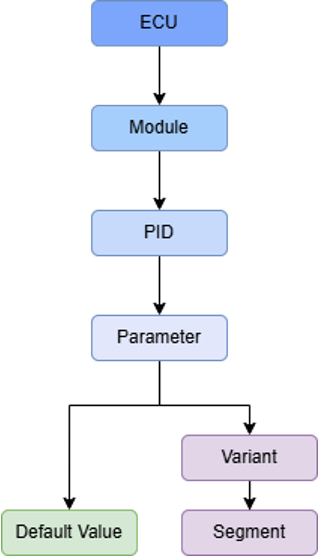
\includegraphics[height=0.4\textheight]{figures/ecu_hierarchy.png}
    \caption{Hierarchical Organization of Automotive Electronic Systems}
    \label{fig:ecu-hierarchy}
\end{figure}

As shown in Figure \ref{fig:ecu-hierarchy}, parameters can either use their default values or be customized through variants and segments. When a parameter is used without customization, its default value is applied. However, when specific vehicle configurations require different parameter settings, variants are created, and segments define the modified parameter values within these variants. This hierarchical structure is not merely organizational but reflects the actual architecture of automotive electronic systems, where software components are modularized for maintainability, reusability, and functional separation. The \ac{CPC}, a central \ac{ECU} in modern trucks, manages critical powertrain functions through thousands of configurable parameters organized into this hierarchical structure \cite{staron2021automotive}.

Parameters themselves have complex characteristics beyond simple values. They can be scalar values, one-dimensional arrays (curves), or multi-dimensional arrays (maps or tables). Each parameter has specific attributes defining its data type, valid range, engineering units, scale factors, and default values \cite{pretschner2007software}. For instance, an engine timing map might be represented as a two-dimensional array where engine speed and load are the independent variables, and ignition timing angle is the dependent variable. This complexity in parameter structure creates specific requirements for the database system designed to manage them.

\subsection{Parameter Variants and Customization}
\label{subsec:parameter-variants}

A fundamental challenge in automotive parameter management is supporting multiple parameter configurations for different vehicle variants, regional requirements, and operating conditions. Rather than maintaining separate complete parameter sets for each configuration, which would lead to significant redundancy, automotive systems implement a variant mechanism that allows selective overriding of parameter values based on specific conditions \cite{staron2021automotive}.

In this approach, each parameter has a default value defined in the baseline configuration. Variants are created to represent specific vehicle configurations or conditions, and segments define modified parameter values within these variants. If no segment exists for a particular parameter in an applicable variant, the default value is used. This approach minimizes redundancy by storing only the modified values rather than complete parameter sets for each configuration \cite{broy2006challenges}.

The lower part of Figure \ref{fig:ecu-hierarchy} illustrates this concept, showing how parameters can follow two paths: either using their default values (left branch) or being customized through variants and segments (right branch). Variants are associated with code rules—boolean expressions that determine when a variant applies based on vehicle configuration codes. For example, a variant might apply only to vehicles with a specific engine type and transmission combination, or to vehicles destined for a particular market with unique regulatory requirements. The code rule evaluation process selects the appropriate variants for a specific vehicle configuration during parameter file generation \cite{staron2021autosar}.

This variant approach creates specific requirements for the database system, which must efficiently store and retrieve variant definitions and segment values while maintaining the relationships between parameters, variants, and segments. The system must also implement a parameter resolution process that correctly applies variants based on vehicle configuration codes, ensuring that the right parameter values are used for each specific vehicle.

\subsection{Release and Phase Management}
\label{subsec:release-phase-management}

Automotive software development follows a structured release process with well-defined phases representing increasing levels of maturity and stability \cite{broy2006challenges}. For parameter management, this translates into a phase-based development process where parameter configurations evolve through sequential stages before being released for production.

\begin{figure}[ht]
    \centering
    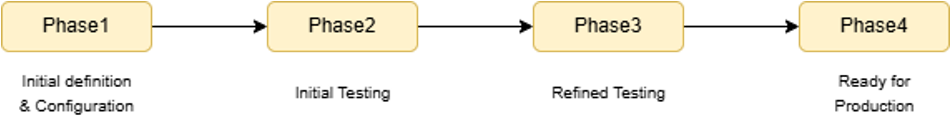
\includegraphics[width=0.85\textwidth]{figures/release_cycle.png}
    \caption{Automotive Parameter Release Cycle}
    \label{fig:release-cycle}
\end{figure}

Figure \ref{fig:release-cycle} illustrates the typical release cycle in automotive parameter development, consisting of bi-annual releases (e.g., "24.1" and "24.3" for first and third quarters of 2024), with each release progressing through four sequential phases: Phase1 (Initial definition \& Configuration), Phase2 (Initial Testing), Phase3 (Refined Testing), and Phase4 (Ready for Production). The diagram shows the linear progression through these phases, with each phase building upon the work completed in the previous phase. Different \acp{ECU} may progress through these phases at different rates, requiring the parameter management system to support concurrent work on multiple phases.

Each phase represents a milestone in the development process with specific activities and quality gates. The Phase1 involves the creation of new parameters and initial configuration. Phase2 and Phase3 involve refinement based on testing feedback, with increasing levels of validation. The Phase4 represents the completed configuration ready for production release \cite{staron2021automotive}.

When a phase transitions to the next stage, parameter configurations are copied forward, establishing a new baseline for continued development. Changes made in earlier phases should propagate to later phases unless explicitly overridden, creating a complex versioning requirement for the parameter management system \cite{pretschner2007software}. Additionally, at specific development milestones, phases may be "frozen" to create stable reference points for documentation and testing, requiring the parameter management system to enforce read-only access to frozen phases while still allowing continued development in active phases.

This phase-based release process establishes specific requirements for the database system's versioning model, which must maintain distinct parameter configurations for each phase while supporting phase transitions, change propagation, and selective freezing. The versioning approach must align with this development process rather than implementing a generic temporal model, ensuring that the system supports the actual workflows used in automotive parameter development.

\section{Database Management Systems}
\label{sec}

\ac{DBMS} serve as the foundation for structured information storage and retrieval. They provide mechanisms for storing, organizing, and accessing data while ensuring integrity, security, and concurrent access \cite{elmasri2015fundamentals}. For the \ac{VMAP} system, selecting an appropriate database approach is critical for meeting the complex requirements of automotive parameter management.

\subsection{Relational Database Management Systems}
\label{subsec:relational-database-management-systems}

\ac{RDBMS} organize data into structured tables composed of rows and columns, based on the relational model proposed by E.F. Codd in 1970 \cite{codd1970relational}. The relational model establishes a mathematical foundation for representing data as relations (tables) with well-defined operations for data manipulation. This approach has dominated database technology for decades due to its solid theoretical foundation and practical advantages for structured data management.

\begin{figure}[ht]
    \centering
    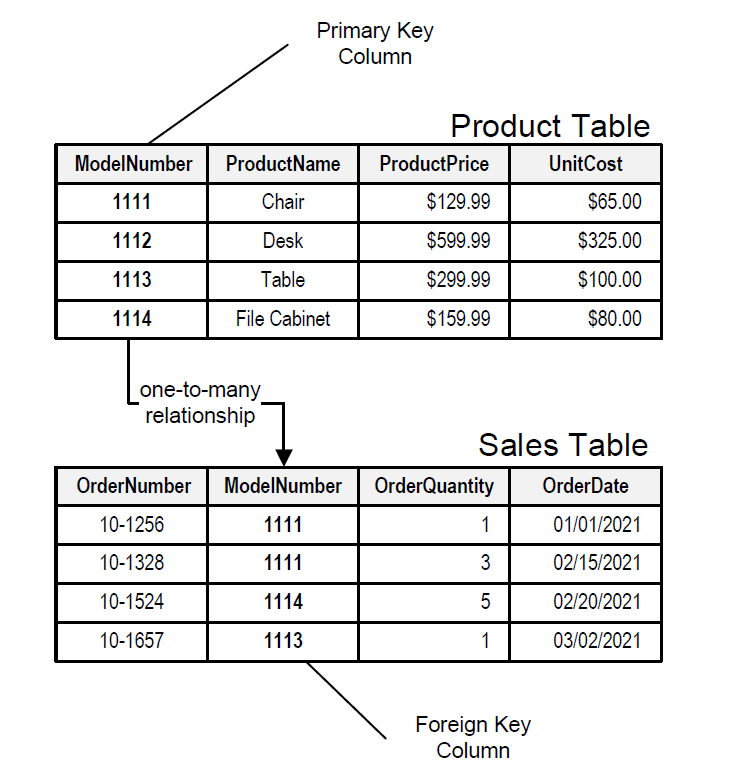
\includegraphics[width=0.85\textwidth]{figures/relational_schema.png}
    \caption{Example of a Relational Schema \cite{noah2024relational}}
    \label{fig:relational-schema}
\end{figure}

Figure \ref{fig:relational-schema} illustrates a practical example of a relational schema with two related tables. The Product Table contains product information with ModelNumber as the primary key, while the Sales Table captures order information with OrderNumber as its primary key. The relationship between these tables is established through the ModelNumber field in the Sales Table, which serves as a foreign key referencing the Product Table. This one-to-many relationship indicates that a single product can appear in multiple sales orders. The diagram clearly shows how primary and foreign keys establish relationships between tables, implementing the referential integrity that ensures consistency across related data.

In relational databases, tables adhere to predefined schemas that specify the structure, data types, and constraints applicable to the data. Each table typically includes a primary key that uniquely identifies each row, while foreign keys establish relationships between tables, implementing the referential integrity that ensures consistency across related data \cite{elmasri2015fundamentals}.

A key strength of relational databases is their adherence to ACID properties (Atomicity, Consistency, Isolation, Durability), which ensure reliable transaction processing. Atomicity guarantees that transactions are treated as indivisible units that either complete entirely or have no effect. Consistency ensures that transactions maintain database integrity by transforming the database from one valid state to another. Isolation prevents interference between concurrent transactions, making them appear as if executed sequentially. Durability ensures that committed transactions persist even after system failures \cite{elmasri2015fundamentals}.

ACID compliance makes relational databases particularly suitable for automotive parameter management, where data integrity and consistency are paramount. Incorrect parameter values could potentially affect vehicle safety and performance, making the strong consistency guarantees of relational databases essential for maintaining data integrity \cite{staron2021automotive}. Additionally, the hierarchical structure of automotive parameter systems—with well-defined relationships between \acp{ECU}, modules, \acp{PID}, and parameters—aligns naturally with the relational model's representation of structured data and relationships.

\subsection{Non-Relational Database Systems}
\label{subsec:non-relational-database-systems}

Non-relational databases, often referred to as \ac{NoSQL} databases, emerged as alternatives to the relational model, particularly for use cases involving large-scale distributed systems, unstructured data, or schema flexibility requirements. Unlike relational databases, NoSQL systems typically sacrifice some aspects of ACID compliance in favor of scalability, flexibility, and performance characteristics suited to specific application domains \cite{bhattacherjee2015principles}.

\begin{figure}[ht]
    \centering
    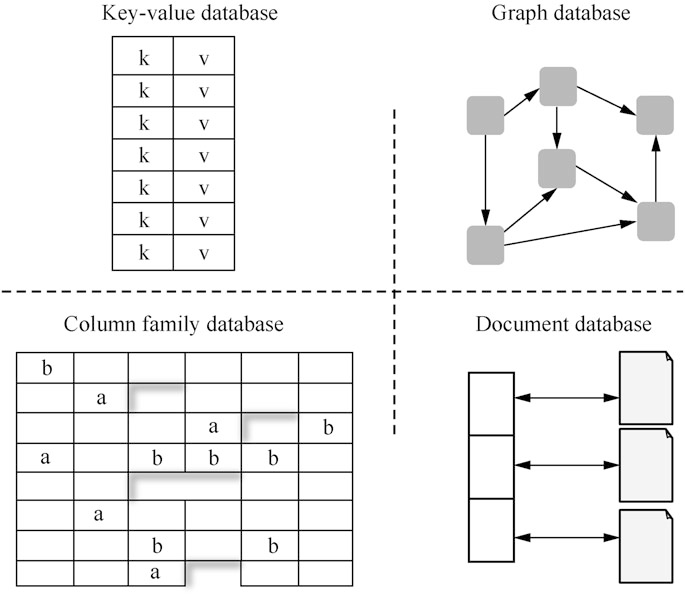
\includegraphics[width=0.85\textwidth]{figures/nosql_types.png}
    \caption{Major Types of NoSQL Databases \cite{gaussdbdatabase}}
    \label{fig:nosql-types}
\end{figure}

Figure \ref{fig:nosql-types} illustrates the four major types of \ac{NoSQL} databases, each with distinct data models and storage approaches. Key-value databases (top-left) store data as simple key-value pairs, offering fast lookups but limited query functionality. Graph databases (top-right) organize data as networks of interconnected nodes and relationships, excelling at representing complex relationships. Column-family databases (bottom-left) store data in column-oriented structures that can efficiently handle sparse data. Document databases (bottom-right) store semi-structured data as documents, typically in formats like JSON or XML, providing schema flexibility while maintaining query capabilities.

NoSQL databases can be categorized into these four types based on their data models: document databases (MongoDB, CouchDB), key-value stores (Redis, DynamoDB), column-family stores (Cassandra, HBase), and graph databases (Neo4j, Amazon Neptune). Many NoSQL systems follow the BASE principle (Basically Available, Soft state, Eventually consistent) rather than ACID, prioritizing availability and partition tolerance over immediate consistency \cite{brewer2000towards}.

While NoSQL databases excel in specific domains such as high-volume web applications, real-time analytics, and social networks, they present challenges for applications requiring complex transactions, strict data integrity, or sophisticated query capabilities across related entities \cite{kleppmann2017conflict}. For automotive parameter management, these limitations make NoSQL systems generally less suitable than relational databases.

The potential for eventual consistency rather than immediate consistency in many NoSQL systems could lead to incorrect parameter configurations being used during development or testing, creating significant risks for vehicle performance and safety. Additionally, the hierarchical nature of automotive electronic systems, with well-defined relationships between entities, aligns naturally with the relational model's approach to representing structured data and relationships. The ability to enforce these relationships through foreign key constraints provides important safeguards against data inconsistency that would be more difficult to implement in many NoSQL systems.

\section{Database Design Methodologies}
\label{sec:database-design-methodologies}

Database design methodologies provide structured approaches to creating efficient, reliable database systems. These methodologies help translate real-world information needs into technical implementations that can store and manage data effectively. This section explores fundamental approaches that form the theoretical foundation for database design, presented in a sequence that follows the natural progression from user requirements to technical implementation.

\subsection{Use Case Modeling}
\label{subsec:use-case-modeling}

Before designing a database structure, it is essential to understand how users will interact with the system. Use case modeling provides a technique for capturing user requirements by identifying who will use the system (actors) and what they need to accomplish (use cases). Developed by Ivar Jacobson, use case modeling has become a cornerstone of requirements analysis in system development \cite{jacobson2004use}.

\begin{figure}[ht]
    \centering
    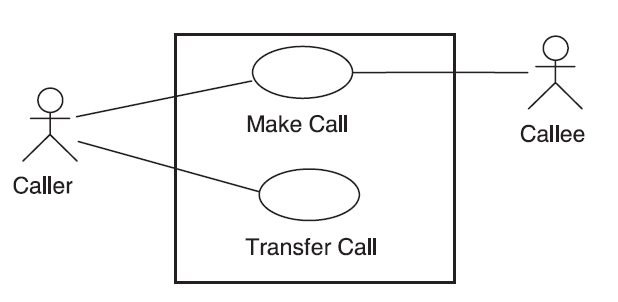
\includegraphics[width=0.7\textwidth]{figures/use_case_diagram.png}
    \caption{Simple Use Case Diagram for a Telephone System}
    \label{fig:use-case-sample}
\end{figure}

Figure \ref{fig:use-case-sample} illustrates a simple use case diagram for a telephone system. The diagram shows two actors, the "Caller" and "Callee," and two use cases, "Make Call" and "Transfer Call." The lines connecting the Caller to both use cases indicate that the Caller can initiate either a direct call or a call transfer, while the Callee is connected only to the "Make Call" use case, indicating their role as the recipient of calls. The rectangle surrounding the use cases represents the system boundary, clearly delineating the functional scope of the telephone system. This visual representation effectively communicates the basic functionality that the system must support, providing a foundation for further design and implementation decisions.

A use case represents a specific goal that an actor wishes to achieve using the system. Actors can be human users with different roles (such as administrators or regular users) or external systems that interact with the database. The collection of all use cases defines the system's functional boundaries—what it must do to satisfy user needs \cite{jacobson2004use}.

Use case diagrams provide a visual representation of these relationships, showing actors as stick figures and use cases as ovals, with lines connecting actors to their associated use cases. This visual format makes the system's purpose accessible to non-technical stakeholders, facilitating communication between developers and users. As noted by Jacobson, "Use cases bridge the gap between the users' and the developers' views of the system" \cite{jacobson2004use}.

For automotive parameter management systems, use case modeling helps identify the different ways in which engineers, documentation specialists, administrators, and other stakeholders need to interact with parameter data. These use cases then inform the database design, ensuring that the resulting structure effectively supports all required operations.


\subsection{Entity-Relationship Modeling}
\label{subsec:entity-relationship-modeling}

After understanding user requirements through use cases, the next step is to model the data itself. \ac{ER} modeling provides a conceptual framework for representing the data structure needed to support the identified use cases. Introduced by Peter Chen in 1976, \ac{ER} modeling has become the most widely used approach for conceptual database design \cite{chen1976entity}.

\begin{figure}[ht]
    \centering
    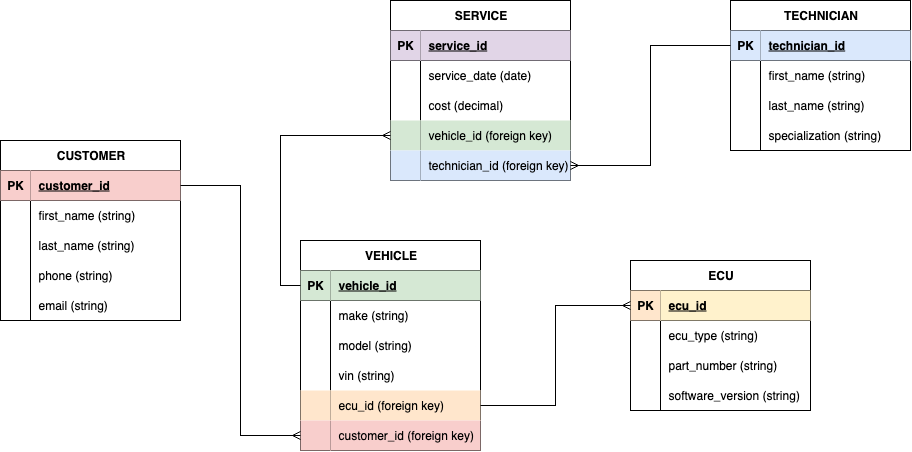
\includegraphics[width=0.95\textwidth]{figures/er_diagram.png}
    \caption{Entity-Relationship Diagram for a Fitness Studio Database}
    \label{fig:er-diagram}
\end{figure}

Figure \ref{fig:er-diagram} presents a detailed \ac{ER} diagram for a fitness studio database. The diagram shows six main entities: Members, Member Signups, Class Schedule, Classes, Types, and Instructors. Each entity is represented as a rectangle containing its attributes, with primary keys clearly labeled at the top of each entity. The diagram uses color coding to visually distinguish different entity types and their related attributes. Foreign key relationships are explicitly shown with connecting lines and arrows pointing to the referenced primary keys, illustrating the database's referential integrity constraints.

The diagram demonstrates several important relational concepts. The Members entity contains basic member information including a unique identifier, name, email, and phone number. The Class Schedule entity serves as a central hub, connecting classes with their instructors and time slots. The Member Signups entity implements a many-to-many relationship between members and scheduled classes, with an additional attribute to track attendance (no\_show). The Classes entity includes a foreign key reference to the Types entity, establishing a categorization system for different class offerings. This comprehensive diagram provides a clear blueprint for database implementation, showing both the structural components and their interrelationships in the fitness studio domain.

\ac{ER} modeling identifies three main components: Entities represent the objects or concepts about which information needs to be stored. In an automotive context, these might include vehicles, \acp{ECU}, parameters, and users. Entities are represented as rectangles in \ac{ER} diagrams. Attributes describe the specific properties or characteristics of each entity. For example, a parameter entity might have attributes like name, value, unit, and description. Attributes are shown as ovals connected to their entity. Relationships describe the associations between entities. For instance, "\acp{ECU} contain parameters" expresses a relationship between \ac{ECU} and parameter entities. Relationships are shown as diamonds connecting the related entities, with cardinality notations indicating how many instances of each entity can participate in the relationship \cite{elmasri2015fundamentals}.

\ac{ER} modeling is particularly valuable for complex domains like automotive systems because it provides a visual representation that stakeholders can understand while being precise enough to guide database implementation. Chen explains that "the \ac{ER} model adopts the more natural view that the real world consists of entities and relationships" \cite{chen1976entity}, making it an intuitive approach for modeling real-world systems.

\subsection{Database Normalization}
\label{subsec:database-normalization}

Once the conceptual model is established through \ac{ER} modeling, database normalization helps refine this model into an efficient, consistent structure. Normalization is a systematic process developed by E.F. Codd that organizes data to minimize redundancy and avoid update anomalies \cite{codd1970relational}.

Normalization proceeds through several "normal forms," each addressing specific types of data inconsistencies:

\ac{1NF} requires that each cell in a table contains only a single value, not a list of values. For example, storing multiple phone numbers in a single field would violate \ac{1NF}. This ensures that data is atomic (indivisible) and can be manipulated consistently.

\ac{2NF} builds on \ac{1NF} by requiring that all non-key attributes depend on the entire primary key, not just part of it. This prevents situations where changing one piece of data requires multiple updates in different places.

\ac{3NF} further refines the structure by requiring that non-key attributes depend only on the primary key, not on other non-key attributes. This eliminates transitive dependencies that can lead to update anomalies \cite{elmasri2015fundamentals}.

For most practical applications, achieving \ac{3NF} provides a good balance between data integrity and system performance. As explained by Date, "Third normal form is considered adequate for most practical purposes; further normalization is usually performed only when necessary" \cite{date2011sql}.

In automotive parameter management, normalization helps organize complex data about \acp{ECU}, modules, and parameters into a structure that maintains consistency while supporting efficient access. For example, normalizing parameter data ensures that when a parameter value changes, that change only needs to be recorded in one place, eliminating the risk of inconsistent values across the database.

\subsection{Role-Based Access Control Models}
\label{subsec:role-based-access-control}

Database systems often contain sensitive information that should not be accessible to all users. \ac{RBAC} provides a structured approach to managing permissions within a database system. Introduced by David Ferraiolo and Richard Kuhn in the 1990s, \ac{RBAC} has become the predominant model for access control in enterprise systems due to its balance of security and administrative simplicity \cite{sandhu1998role}.

The core concept of \ac{RBAC} is that permissions are associated with roles, and users are assigned to appropriate roles rather than being granted permissions directly. A role represents a specific function within an organization, such as ``administrator,'' ``engineer,'' or ``analyst.'' Each role is granted a set of permissions that allow users assigned to that role to perform specific operations on database objects like reading, creating, updating, or deleting records \cite{ferraiolo2011policy}.

This structure provides several important advantages over direct permission assignment. First, it simplifies administration by allowing permissions to be managed at the role level rather than the individual user level. When a new user joins the organization, they can simply be assigned to the appropriate roles rather than requiring configuration of individual permissions. Second, it improves security by implementing the principle of least privilege, ensuring that users have only the permissions necessary for their specific responsibilities which reduces the risk of unauthorized access or accidental data modifications \cite{sandhu1998role}.

The theoretical foundation of \ac{RBAC} includes several key components: users (individuals who need access to the system), roles (collections of permissions that correspond to job functions), permissions (defined operations on specific resources), and sessions (temporary bindings between users and their assigned roles). These components provide a flexible framework for implementing access control policies tailored to specific organizational needs while maintaining a clear separation between users and permissions through the role abstraction \cite{sandhu1997arbac97}.


\subsection{Version Control for Databases}
\label{subsec:database-versioning}

Version control for databases addresses the challenge of tracking changes to data structures and content over time. Unlike traditional file-based version control systems designed for source code, database versioning must maintain complex relationships between entities while preserving historical states and supporting evolution through distinct development stages \cite{bhattacherjee2015principles}.

Several approaches have emerged for implementing version control in database systems. The snapshot approach captures complete database states at specific points in time, providing simple retrieval of historical states but potentially consuming significant storage resources. The change-based approach records only modifications to database content, reducing storage requirements but requiring reconstruction of historical states through the application of change records \cite{bhattacherjee2015principles}.

The temporal approach extends traditional database structures with time dimensions, enabling direct querying of historical states through time-based predicates. This approach typically introduces valid time (when facts are true in the real world) and transaction time (when facts are recorded in the database) dimensions, allowing sophisticated historical analysis but adding complexity to schema design and query formulation \cite{snodgrass1999developing}.

Phase-based versioning represents a domain-specific approach that aligns database versioning with development phases rather than continuous time. This approach explicitly models development stages as first-class entities in the database schema, associating data with specific phases rather than temporal timestamps. According to Bhattacherjee et al., "Domain-specific versioning approaches often provide better performance and usability than generic temporal database techniques when tailored to specific application requirements" \cite{bhattacherjee2015principles}.


\subsection{Temporal Database Concepts}
\label{subsec:temporal-database-concepts}

Many applications, including automotive parameter management, need to track how data changes over time. Temporal database concepts address these requirements by providing mechanisms for managing time-varying data. Unlike traditional databases that store only the current state, temporal databases maintain historical states and support queries based on time dimensions \cite{snodgrass1999developing}.

\begin{figure}[ht]
    \centering
    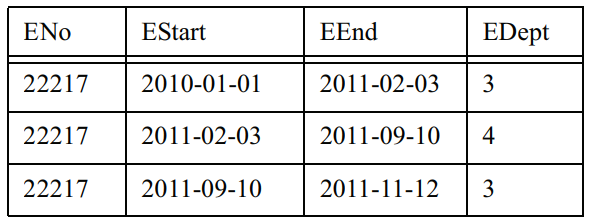
\includegraphics[width=0.8\textwidth]{figures/temporal_database.png}
    \caption{Temporal Table Tracking Employee Department History}
    \label{fig:temporal-database}
\end{figure}

Figure \ref{fig:temporal-database} illustrates a temporal database table that tracks an employee's department history over time. The table contains four columns: ENo (Employee Number), EStart (employment start date in a department), EEnd (employment end date in a department), and EDept (department identifier). The example shows the complete employment history of employee number 22217, who moved between departments over time. The first row indicates that the employee started in department 3 on January 1, 2010, and remained there until February 3, 2011. The second row shows that on February 3, 2011, the employee transferred to department 4, where they stayed until September 10, 2011. The third row demonstrates that on September 10, 2011, the employee returned to department 3, where they remained until November 12, 2011.

This temporal table implementation enables tracking of the complete history of the employee's department assignments without overwriting previous records. Each row represents a specific period during which the employee belonged to a particular department, with non-overlapping time intervals. The start date of each subsequent record matches the end date of the previous record, ensuring continuity in the historical record. This approach to temporal data storage supports historical queries like "Which department did employee 22217 belong to on March 15, 2011?" by evaluating which row's time interval (EStart to EEnd) contains the query date. Such temporal structures are essential for maintaining comprehensive historical records in domains where tracking changes over time is critical, such as automotive parameter management.

Temporal databases typically support two key time dimensions. Valid time represents when facts are true in the modeled reality—for example, when a particular parameter configuration becomes active in a vehicle. Transaction time represents when facts are recorded in the database—for example, when a parameter value was updated in the system. Databases that support both dimensions are known as bi-temporal databases \cite{kulkarni2012temporal}.

Temporal database implementations often use specialized table structures called temporal tables. These tables extend traditional table structures with additional timestamp columns that define the time periods during which each record is valid. For example, a temporal parameter table might include ValidFrom and ValidTo columns that define when each parameter value is applicable, allowing the database to maintain a complete history of parameter changes \cite{salzberg1999comparison}.

Kulkarni and Michels explain that "temporal tables provide a systematic way to track and query historical data without requiring application-level version management" \cite{kulkarni2012temporal}. This capability is particularly valuable in regulated industries like automotive development, where traceability and auditability of parameter changes are essential for compliance and quality assurance.

In automotive parameter management, temporal database concepts can support critical requirements such as tracking parameter evolution throughout the development lifecycle, maintaining historical records for diagnostic and compliance purposes, and enabling historical analysis to understand how parameter configurations have evolved over time. These capabilities form an important theoretical foundation for designing systems that manage time-sensitive data in complex domains.

\subsection{Strategic Denormalization}
\label{subsec:strategic-denormalization}

While normalization provides a theoretical foundation for database integrity, practical database design often requires balancing normalization principles with performance considerations. Strategic denormalization involves deliberately introducing controlled redundancy to improve performance for specific operations \cite{bhattacherjee2015principles}.

Consider a fully normalized database where information about parameters, their modules, and their \acp{ECU} is stored in separate tables. To retrieve a parameter with its associated module and \ac{ECU} information would require joining all three tables—an operation that becomes increasingly expensive as the database grows. In cases where this retrieval happens frequently, storing the module and \ac{ECU} names directly in the parameter table (introducing controlled redundancy) could significantly improve performance \cite{schwartz2012high}.

Molinaro emphasizes that "denormalization is not about abandoning normalization principles, but about making strategic exceptions for performance reasons" \cite{molinaro2005sql}. These exceptions should be carefully documented and justified based on specific performance requirements.

For automotive systems, where both data integrity and query performance are critical, finding the right balance between normalization and strategic denormalization is essential. This balance ensures that parameter data maintains consistency while providing the performance needed for engineering workflows.

\subsection{Conceptual, Logical, and Physical Design Levels}
\label{subsec:design-levels}

Database design typically proceeds through three levels of abstraction, allowing designers to manage complexity by focusing on different aspects at each stage:

Conceptual design focuses on what data needs to be stored, without concern for implementation details. The ER model created at this stage captures entities, attributes, and relationships from a business perspective, providing a foundation that both technical and non-technical stakeholders can understand \cite{elmasri2015fundamentals}.

Logical design transforms the conceptual model into structures specific to the chosen database model (typically relational), defining tables, columns, keys, and relationships. This stage applies normalization principles to refine the structure, independent of any specific database system \cite{elmasri2015fundamentals}.

Physical design addresses how the logical design will be implemented in a specific database management system, considering factors like storage structures, indexing strategies, and access methods. This stage optimizes the design for performance based on anticipated usage patterns \cite{obe2017postgresql}.

Moving through these levels allows database designers to progressively refine the database structure, addressing different concerns at each stage. As Elmasri and Navathe observe, "The separation of conceptual, logical, and physical design allows database designers to focus on the appropriate level of abstraction at each stage" \cite{elmasri2015fundamentals}.

For automotive parameter management, this layered approach helps manage the complexity of the domain, ensuring that the resulting database effectively supports both the business requirements (storing and managing parameter configurations) and the technical requirements (performance, scalability, and maintainability).